\chapter{Background Theory - Fluid Dynamics}
\label{chap:Theory-CFD}
\section{Problem Definition}
The objective of the thesis is to develop a GNN-based surrogate model to understand the jet deflection caused by Coanda effect in a High-speed Orienting Momentum with Enhanced Reversibility (HOMER) nozzle developed by Trancossi and Dumas \cite{trandum}, which is used in aerospace and industrial applications. The HOMER nozzle is designed to produce a controllable and selective deviation of a synthetic jet generated by mixing two primitive jets, without requiring any mechanical part but solely by taking advantage of the Coanda effect. The general construction of the nozzle is depicted in \ref{fig:nozzle}. As we can see from the figure, the nozzle has two inlets fed by two impinging jets followed by a convergence zone or septum where mixing of the flows occurs. The mixing of flows generates a synthetic outflow jet, which can be controlled by modifying the momentums of the primitive jets. Next to the convergence zone is the outflow mouth with curved walls connected to two convex Coanda surfaces on the top and bottom.
\begin{figure}[ht]
  \centering
  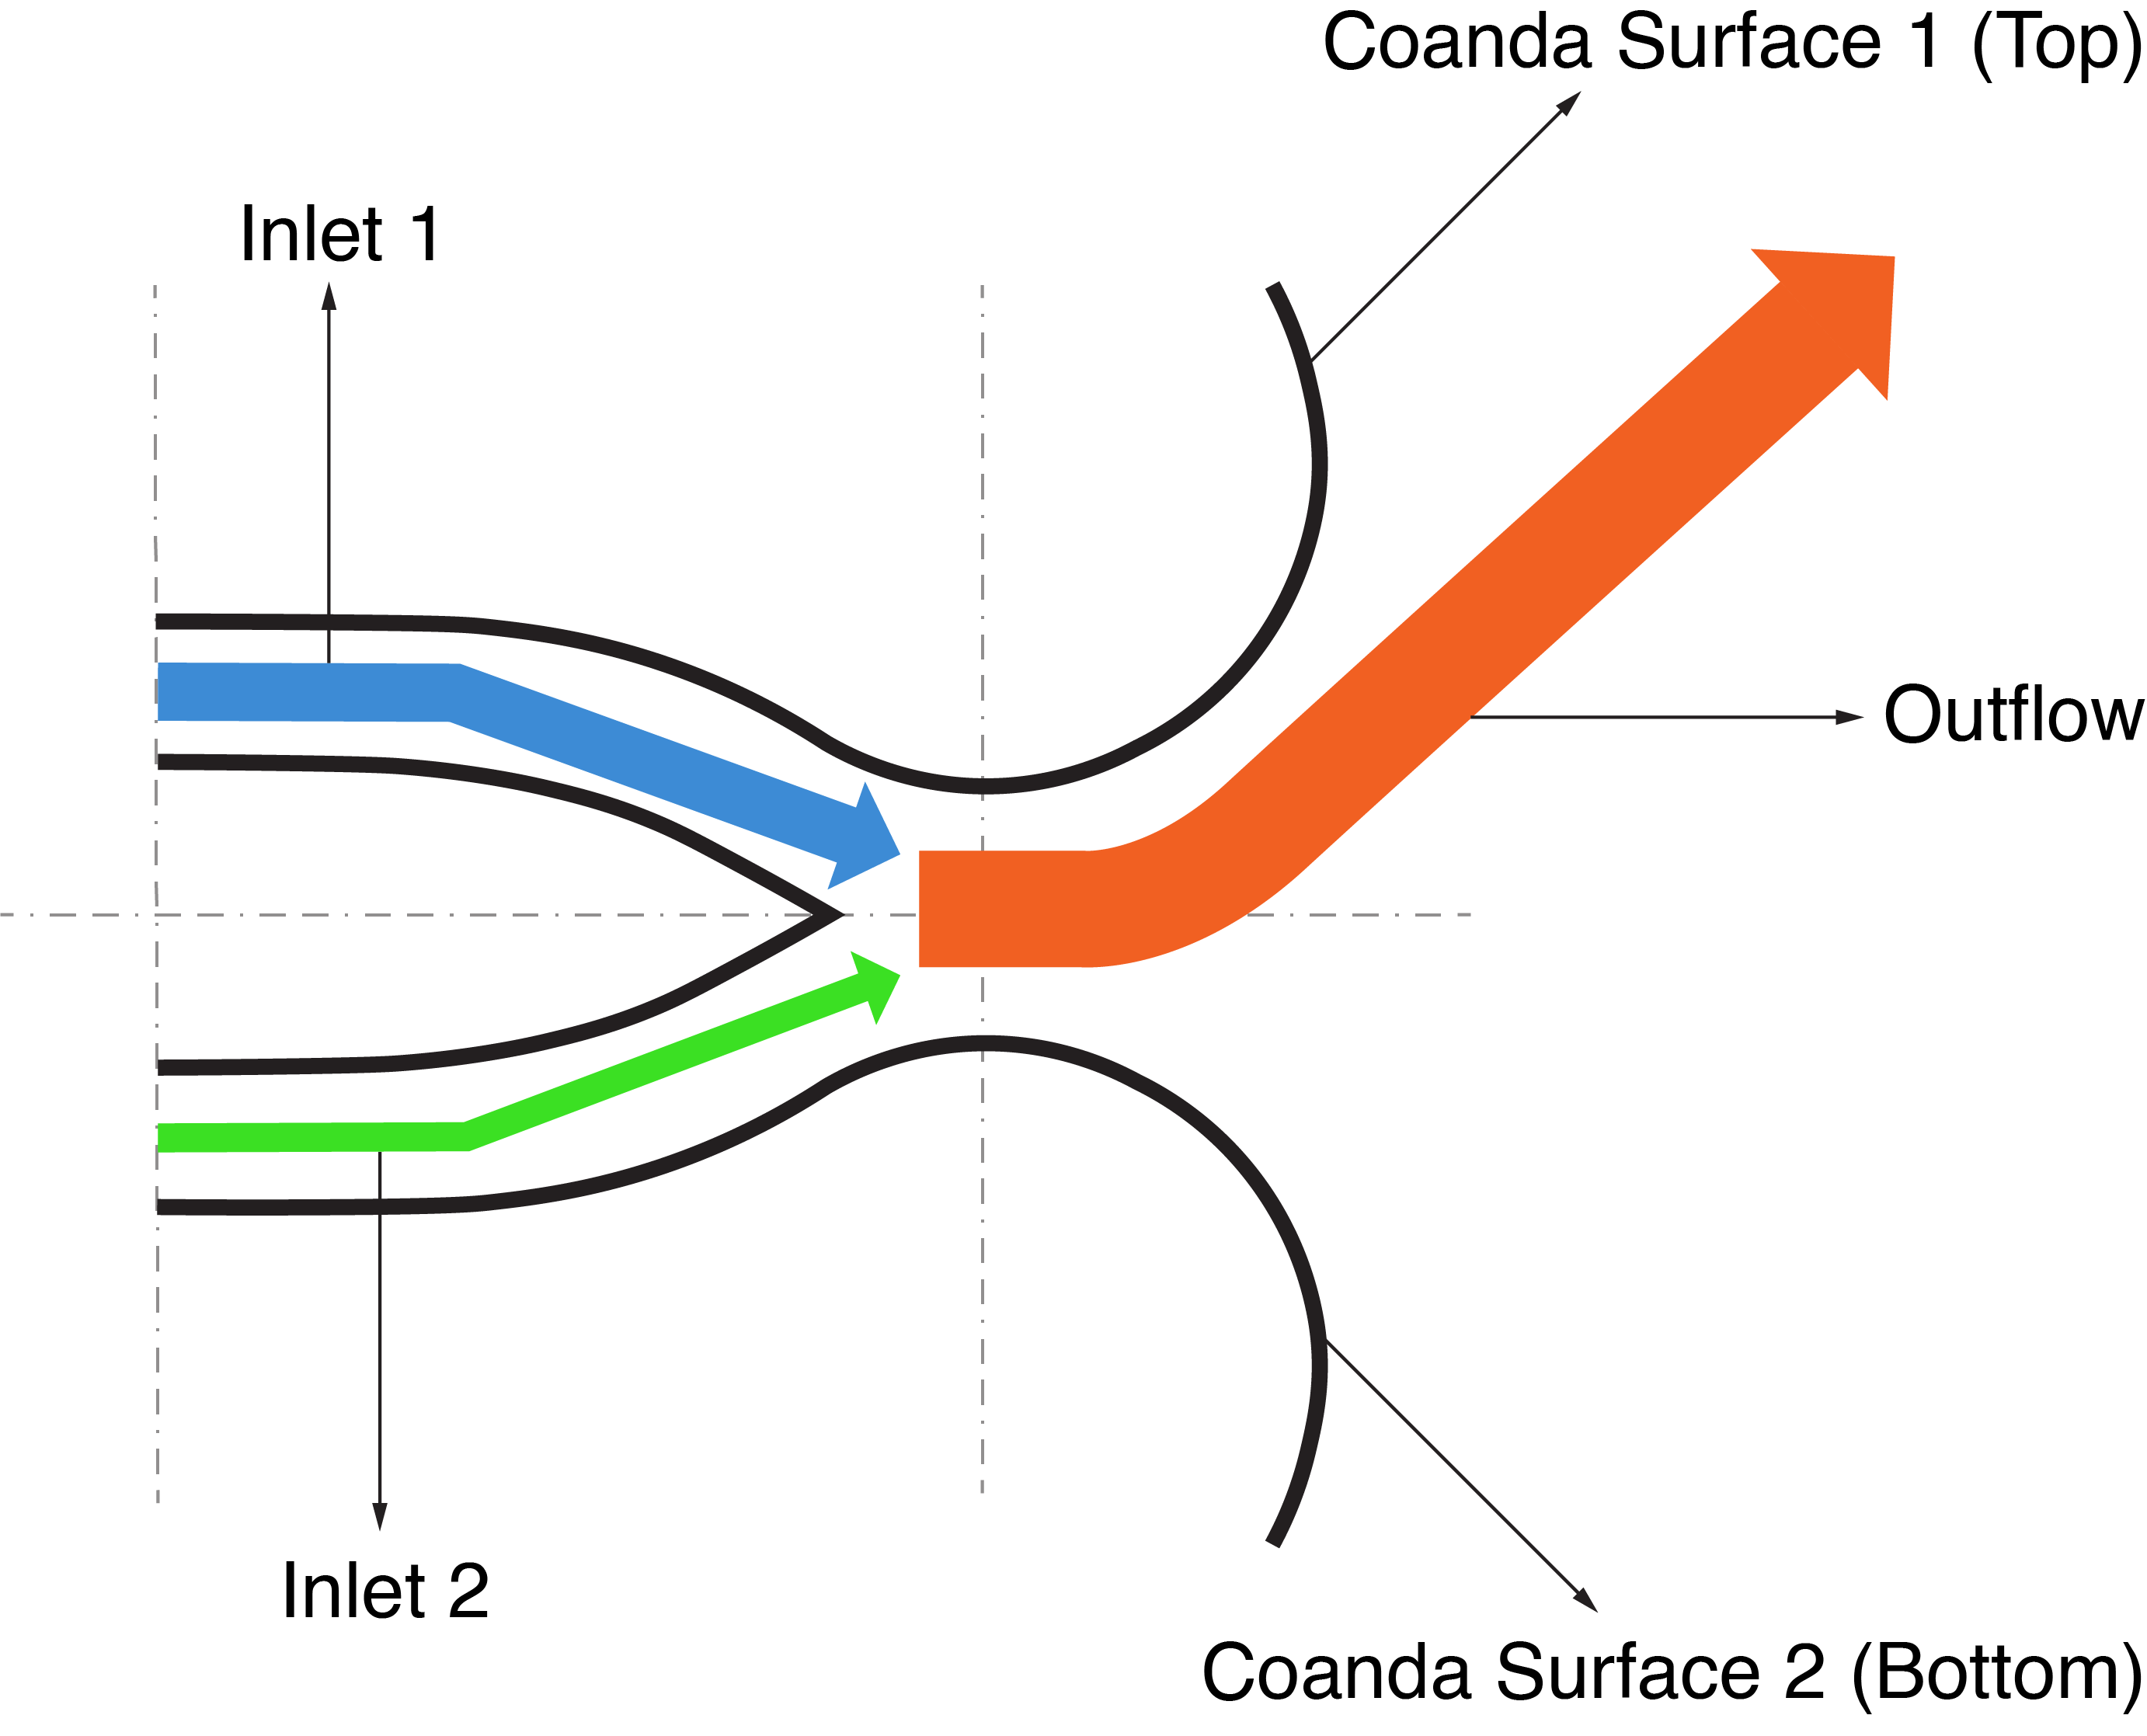
\includegraphics[width=10cm]{images/Theory-CFD/nozzle.png}
  \caption{Nozzle Architecture}
  \label{fig:nozzle}
\end{figure}
The system requires a minimum operating condition of the primitive jets to ensure effective mixing. The impinging jets must have velocities high enough to generate a synthetic jet of Reynolds number greater than 50000 at the outlet mouth. To guaranteee optimum operation, the Reynolds number at the outlet must exceed 10000. In the case of lower Reynolds numbers the system behavior is unpredictable. 
\subsection{Coanda Jet Deflection in the HOMER nozzle}
The Coanda effect is the tendency of a stream of fluid emerging from an orifice to follow an adjacent flat or curved surface and to entrain fluid from the surroundings so that a region of lower pressure develops. In simple terms, it is the tendency of a fluid to adhere to and stay attached to the walls of a convex surface, which is demonstrated in \ref{fig:Coanda}. Different fluid dynamic effects concur to create the so called “Coanda effect”. In particular it has been completely formulated in as the combination of three effects: the boundary layer effect, the tendency of a fluid jet approaching a curved surface to remain attached to the surface; the adhesion effect, the ability of a fluid jet to adhere to a nearby surface; the attraction effect, the tendency of jet flows over convex curved surfaces to attract surrounding fluid and increase more rapidly than that of plane wall jets. Newman \cite{newman} has investigated a two-dimensional, incompressible, turbulent jet flowing around a circular cylinder. He has demonstrated that Coanda adhesion to a curved surface is dependent on the equilibrium of forces applied on the fluid. Adhesive motion on a curved surface involves centrifugal force and radial pressure, with contact pressure decreasing due to viscous drag upon jet exit. This pressure differential propels fluid along the curved surface until surface pressure matches ambient pressure, causing detachment. Viscous effects increase jet thickness and decrease mean velocity along the curved surface due to adverse pressure gradient. While inviscid flows can adhere via centrifugal forces, viscous effects lead to jet separation.
\begin{figure}[ht]
    \centering
    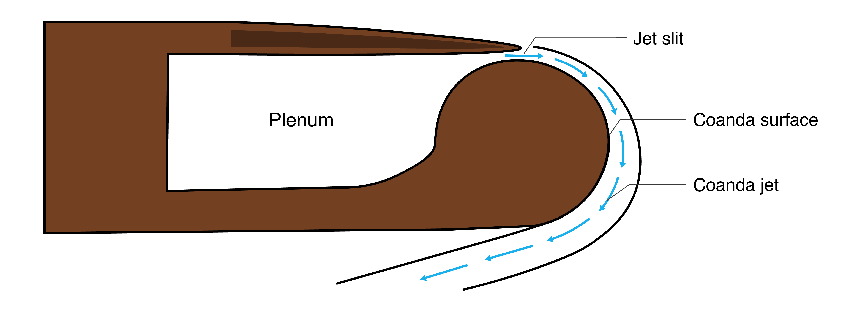
\includegraphics[width=10cm]{images/Theory-CFD/Coanda-effect.png}
    \caption{Coanda Effect}
    \label{fig:Coanda}
  \end{figure}
\section{Flow Simulation}
The Navier-Stokes equations can be used to mathematically model the flow field of an incompressible Newtonian fluid within the computational domain. 
\ref{fig:Domain} shows the computational domain for our fluid flow problem. We consider the same homogenous fluid for both the primitive jets, that is, streams with the same chemical and physical properties ($\rho$ = constant). The fluid in consideration is air in ideal gas conditions. 
\begin{figure}[ht]
  \centering
  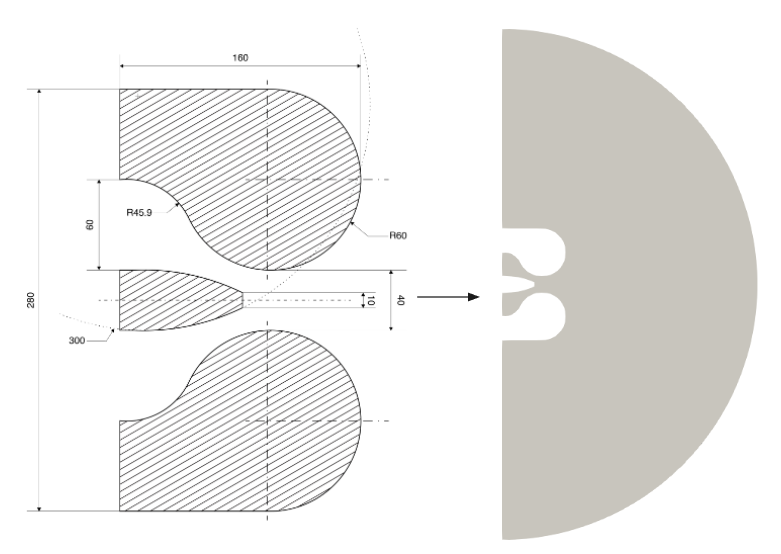
\includegraphics[width=7cm]{images/Theory-CFD/Flow Domain.png}
  \caption{Computational Flow Domain}
  \label{fig:Domain}
\end{figure}
\begin{equation}
  \begin{aligned}
  &\frac{\partial u_i}{\partial x_i}=0\\
  &\frac{\partial u_i}{\partial t}+u_j \frac{\partial u_i}{\partial x_j}=\frac{-1}{\rho} \frac{\partial p}{\partial x_i}+\nu \frac{\partial^2 u_i}{\partial x_j^2}
  \end{aligned}
  \end{equation}
where, $u_i$ is the flow velocity in the spatial direction $x_i$, $\nu$ is the kinematic viscosity, $\mu$ is the dynamic viscosity ($\nu = \mu / \rho$), $\rho$ is the density of the fluid, $p$ is the pressure. A velociy profile from a fully-developed turbulent plane channel flow is prescribed as inlet velocities at $\partial{\Omega_{in}}$. No-slip boundary conditions are applied at the walls $\partial{\Omega_{wall}}$. Zero-gradient Neumann boundary condition is imposed on the flow quantities at outlet.\\
Turbulence, characterized by its unsteady, highly irregular, rotational and energy dissipative behaviors at high Reynolds numbers, engenders minute fluctuations in velocity, pressure, and temperature across varying scales. While a direct numerical solution (DNS) could theoretically capture these fluctuations by solving the Navier-Stokes equations, the immense computational resources required render it impractical for most engineering simulations. 
% Turbulence modelling serves as a pragmatic approach to predict time-averaged fields without needing to resolve every turbulent detail.
Turbulence modelling using RANS (Reynolds-Averaged Navier-Stokes) equations offers a practical compromise by solving time-averaged equations for steady-state or unsteady (URANS) flows. RANS relies on turbulence models to account for unresolved turbulence effects, allowing for efficient simulations of complex engineering systems without resolving every turbulent detail. The underlying principle is to consider the flow as the sum of mean flow and turbulent/fluctuating component. For a steady-state flow field, Reynolds decomposition is applied to flow quantities like the flow velocity, expressed as $u_i = U_i + u_i^{\prime}$ where $U_i$ is the mean velocity and $u_i^{\prime}$ is the fluctuating turbulent component. The Reynolds averaging process introduces an additional term to the NSE known as Reynolds stress.  By substituting the averaged quantities in the Navier-Stokes equation, we obtain the RANS equations for our steady-state, 2D incompressible flow as,
\begin{equation}
  \begin{aligned}
  \frac{\partial u_i}{\partial x_i}=0 \\
  u_j \frac{\partial u_i}{\partial x_j}=\frac{1}{\rho}\frac{\partial}{\partial x_j}     \left[-p \delta_{i j}+\mu \left(\frac{\partial u_i}{\partial x_j}+\frac{\partial u_j}{\partial x_i}\right) - \rho u'_i u'_j \right]
  \end{aligned}
\end{equation}
where $- \rho u_i^{\prime} u_j^{\prime}$ is called the Reynolds stress tensor and represents the effect of the small-scale turbulence on the average flow. Here, $u$ and $P$ are the averaged flow quantities $\langle u \rangle $ and $\langle P \rangle $ but the averaged notation $\langle ... \rangle $ has been omitted for convenience. The RANS equations have no unique solution because they are not in a close form, the unknowns being more than the equations. Thus, additional equations are needed to close the problem. The most common strategy used in CFD is to relate the Reynolds stress to the shear rate by the Boussinesq relationship:
\begin{equation}
  u_i^{\prime} u_j^{\prime}=2 \frac{\mu_t}{\rho} S_{i j} \quad \text { with } \quad S_{i j}=\frac{1}{2}\left(U_{i, j}+U_{j, i}\right)
\end{equation}
where $\mu_t$ is the turbulent viscosity, which is usually computed from the turbulence models. Some of the RANS-based turbulence models are outlined below: 
\begin{enumerate}
  \item The Spalart-Allmaras model is a one-equation model that is computationally efficient. It solves for a single variable, the turbulent viscosity, using a transport equation derived from the RANS equations. 
  % This model is particularly suited for aerodynamic flows, offering reliable predictions with reduced computational cost.
  \item The $\text{k}-\epsilon$ model resolves turbulence through two transport equations: one for turbulent kinetic energy ($\text{k}$) and another for the rate of dissipation of turbulent kinetic energy ($\epsilon$). 
  % These equations govern the behavior of turbulence in a wide range of flows, from boundary layers to free shear flows.
  \item The $\text{k}-\omega$ model is another two-equation turbulence model that features transport equations for turbulent kinetic energy and specific rate of turbulence dissipation ($\omega$). This model is particularly advantageous in accurately predicting near-wall flows and is less susceptible to numerical issues than the $\text{k}-\epsilon$ model in adverse pressure gradient regions. 
  \item The $\text{k}-\omega $  SST (Shear-Stress Transport) model combines aspects of the $\text{k}-\epsilon$ model near walls and the $\text{k}-\omega$ model away from walls to provide accurate predictions in both regions. The $\text{k}-\omega \text{SST}$ model is particularly suitable for boundary layer flows, capturing the near-wall behavior accurately while providing robust predictions in the outer flow regions. Its versatility and computational efficiency make it a popular choice for a wide range of engineering applications.
\end{enumerate}
For the purposes of this work, the $\text{k}-\omega$ SST turbulence model has been adopted.\\
Numerical analysis on PDEs - in our case, the RANS equations is performed by discretizing the continuous domain into a discrete setup which results in a system of algebraic equations which are usually linear systems that can be solved by iterative techniques such as Jacobi or Gauss-Seidel. Multigrid methods are another class of iterative numerical techniques used to solve discretized PDEs efficiently for large-scale computational problems. They employ a hierarchy of grids with varying levels of resolution, combining coarse and fine grids to accelerate convergence. By addressing error components on multiple scales, multigrid methods effectively smooth out high-frequency errors while retaining accuracy, making them particularly suitable for problems with smooth solutions or complex geometries. \\
Some commonly used discretization techniques are Finite Difference Method (FDM), Finite Element Method (FEM) and Finite Volume Method (FVM). All three methods end up solving one (or several) system(s) of linear equations to compute an approximate numerical solution of the PDE at hand. And for all three methods, these linear systems are sparse, and the equation for an unknown $u_i$ involves only a few neighbors of point $i$. Overall, FDM is mostly used for geometries that can be discretized by structured grids (e.g., rectangles), while FEM and FVM are more suitable for complex domains. \\
The finite volume method discretizes PDEs by dividing the computational domain into finite volumes or cells. It conservatively approximates integral forms of conservation laws within each cell. The method calculates fluxes across cell interfaces, preserving conservation principles, making it particularly suited for problems involving fluid flow, heat transfer, and other conservation phenomena. As FVM is based on the integral formulation of a conservation law, it is mainly used to solve PDEs in fluid dynamics, which involves fluxes of the conserved variable. In this thesis, we are only interested in the discretization of general PDEs defined on a complex geometry using FVM, which is the most widely used discretization approach in CFD solvers. 
% In the case of non-linear systems arising from discretization, linearization schemes are required to convert the non-linearity into a sequence of linear systems: a sequence of linearized equations is solved iteratively, converging to the solution of the non-linear system. 
